\section{Interfacing with applications}

The ultimate goal of the \vtkm work for the ECP was to provide scientists with the tools needed to understand large amounts of data and make scientific discoveries.
The previous sections of this paper describe the efforts for making these tools available.
This section provides some examples of applying \vtkm and its companion enabling technologies to real-world science problems, which often happens through the visualization tools described in the previous section.

%% \ken{
%%   Each subsection should be up to 2/3 pages plus have images up to 1/2 page.
%%   (3.5 pages total.)
%%   The section should start with a layperson overview of what the domain problem is, what scientists are doing to study the problem.
%%   The section should then explain how visualization fits in to help.
%%   Explain the technical solution of how \vtkm was integrated into the system and describe the final result.
%%   The section may repeat for multiple things that were done.
%%   For example the fusion reactor could first talk about in situ images and then Poincar\'{e} plots.
%%   The laser wakefields could talk about deliver of in situ images via Ascent and then about the customized particle advection.
%%   The final section will be a little different in that it will iterate over multiple science domains.
%% }


\begin{figure*}[ht]
  \begin{tabularx}{\textwidth}{l@{}X@{}r}
    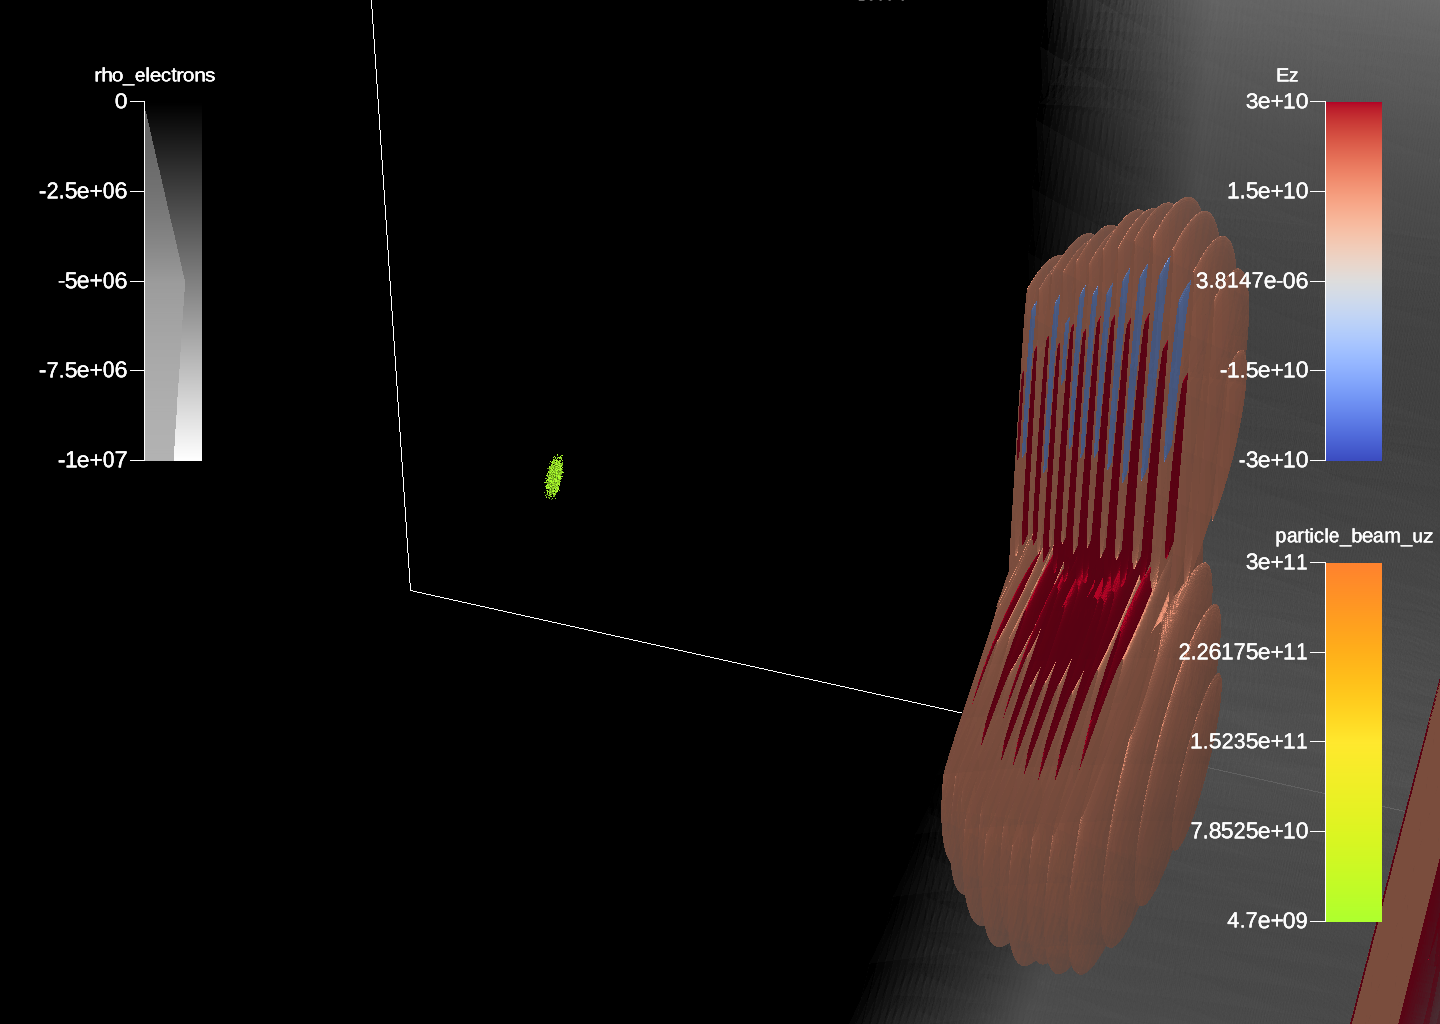
\includegraphics[width=0.475\textwidth]{ez_007050}
    & &
    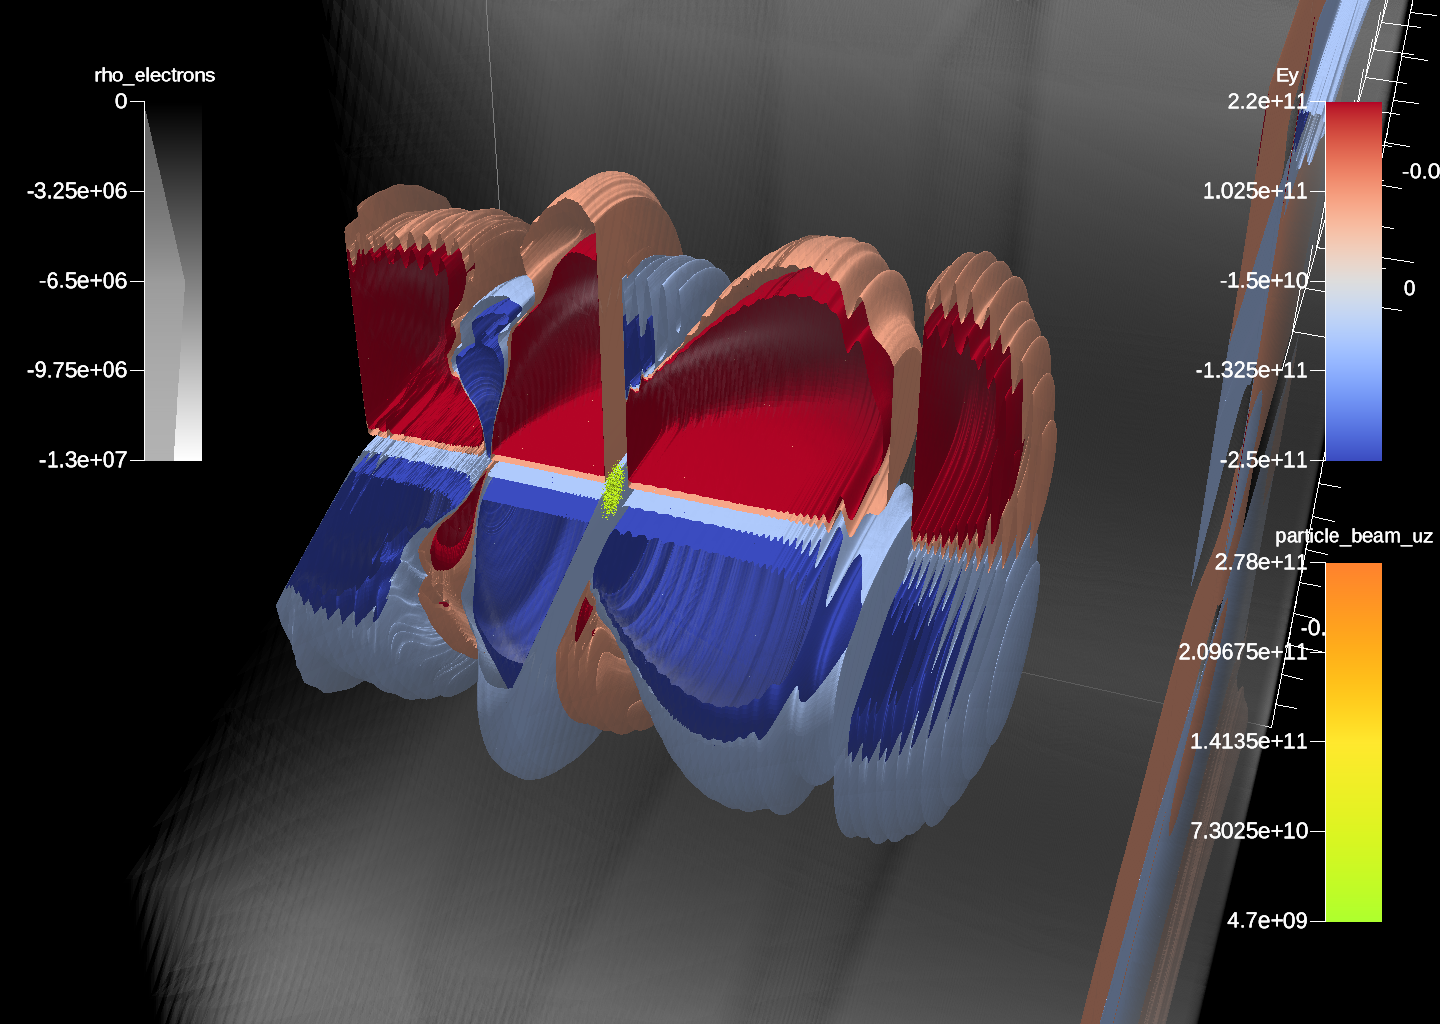
\includegraphics[width=0.475\textwidth]{ey_009300}
    \\
    \begin{minipage}{0.475\textwidth}
      \caption{
        WarpX in-situ visualization of a laser-wakefield accelerator on 4,416 GCDs across 552 nodes of Frontier using Ascent and \vtkm.
        The image depicts an early time step of the simulation at high resolution.
        \label{fig:warpx_highres}
      }
    \end{minipage}
    & &
    \begin{minipage}{0.475\textwidth}
      \caption{
        WarpX in-situ visualization of a laser-wakefield accelerator on 552 GCDs across 69 nodes of Frontier using Ascent and \vtkm.
        The image depicts a later time step of the simulation at low resolution.
        \label{fig:warpx_lowres}
      }
    \end{minipage}
  \end{tabularx}
\end{figure*}

\subsection{Laser wakefield acceleration}\label{sec:warpx}

%\assign{Axel, Abhi}~%
%
%\defcitealias{FedeliHuebl2022}{Fedeli, Huebl et al. (2022)}
%\citepalias{FedeliHuebl2022}
%
WarpX is a particle-in-cell simulation code and was awarded the 2022 ACM Gordon Bell Prize~\citep{FedeliHuebl2022}.
As part of the ECP, WarpX was developed as a new application to succeed its predecessor, Warp~\citep{Vay2013}, with the goal of studying advanced particle acceleration in laser-driven plasma wakefields in an effort to advance future high-energy physics colliders~\citep{Albert2021}.
Beyond that, WarpX is used to describe kinetic physics in particle accelerators, laser-plasmas, fusion devices, inertial confinement fusion, and astrophysical plasmas and to model microelectronics~\citep{Yao2022}.

\begin{figure*}[ht]
  \centering
  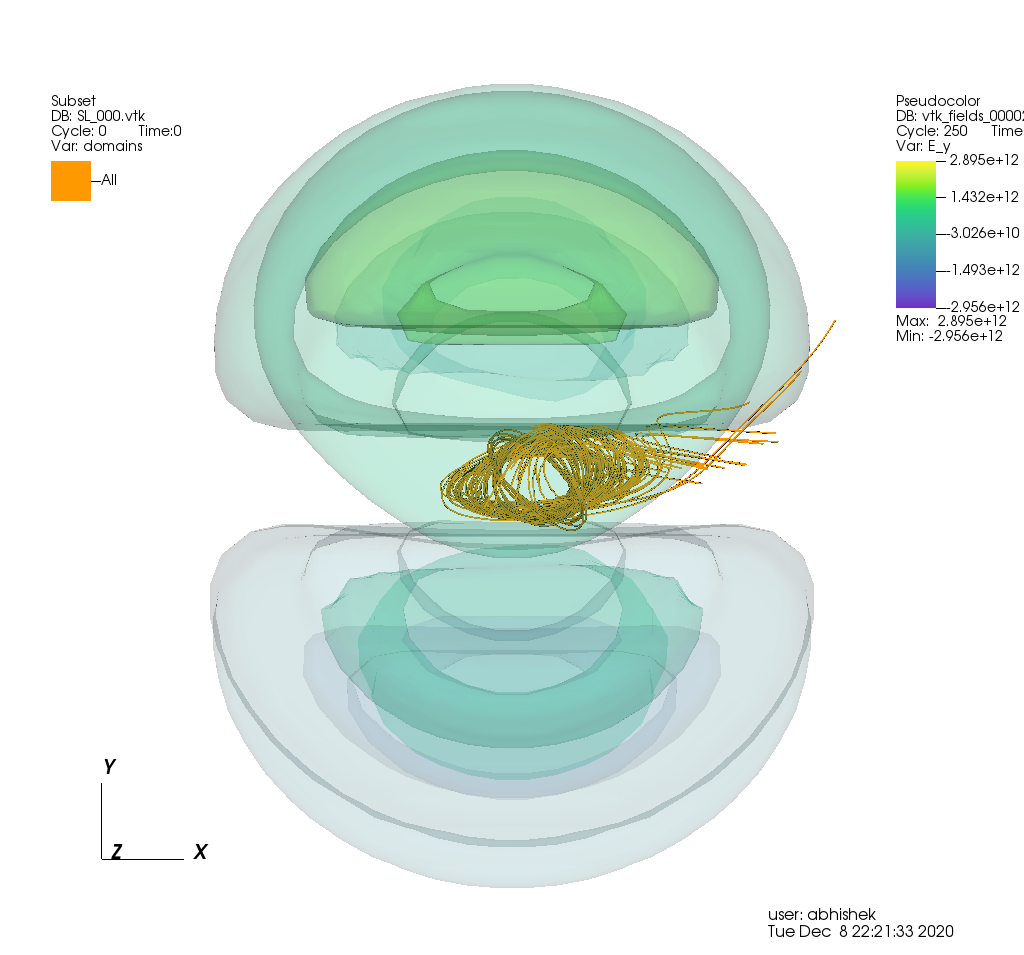
\includegraphics[width=0.49\linewidth]{lwfa_particle_advection_front}%
  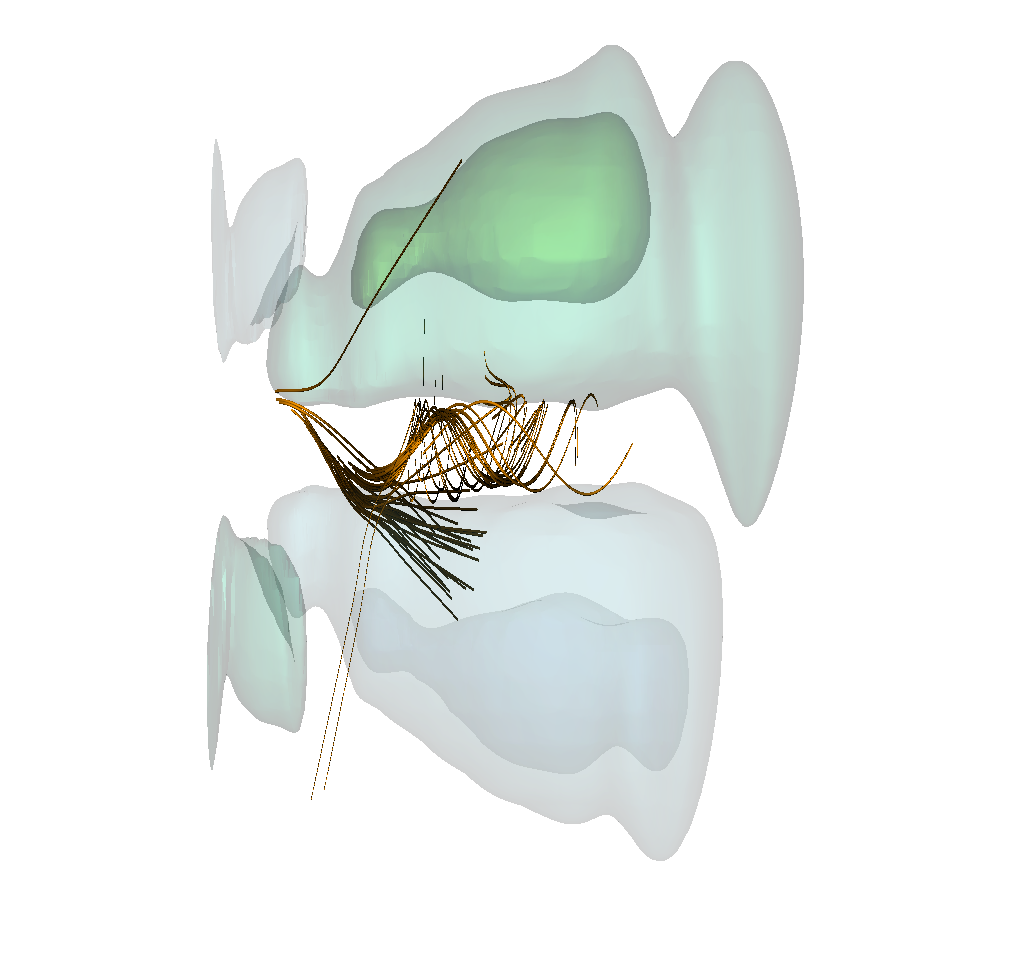
\includegraphics[width=0.49\linewidth]{lwfa_particle_advection_side}
  \caption{Side and front views of a laser wakefield with an injected electron bunch.
  Particles are advected from \emph{a single snapshot} of the simulation in \vtkm.}
  \label{fig:lwfa_particle_advection}
\end{figure*}

Figures \ref{fig:warpx_highres} and \ref{fig:warpx_lowres} are in-situ renderings of a \emph{staged} laser wakefield accelerator in a boosted reference frame~\citep{Vay2011}.
An electron beam (orange-green) is accelerated to the right through multiple stages to high energies.
In the plasma stages (gray), the strong traversal focusing fields are shown in red-blue.

In the staging approach, a particle beam is accelerated through multiple plasma elements.
In each stage, an ultra-intense laser pulse excites a plasma wakefield.
This depletes the laser pulse's energy and generates very strong electric fields in the plasma wake, which can be used to accelerate an injected electron beam.
The acceleration itself can be 3--4 orders of magnitude more compact than relying on state-of-the-art radio-frequency accelerator elements.
Besides increased beam energy, physicists study how to preserve beam properties essential for transport, focusing (e.g., emittance), and applications (e.g., charge and current).

WarpX features advanced techniques such as GPU-acceleration for three vendors, mesh-refinement capabilities, dynamic load balancing, and unique advanced numerical solvers.
WarpX relies on multi-level parallelization: coarse parallelization uses block-structured domain decomposition with MPI using the AMReX library~\citep{Zhang2019}, and compute acceleration leverages CUDA/HIP/SYCL or OpenMP so that the simulations can scale on large, massively parallel HPC systems.

If WarpX relied on only traditional post-processing workflows for the visualization of the dynamics of exascale simulations, the resulting multi-petabyte scale output per simulation would severely limit the available snapshots and/or level of detail to visualize.
Addressing this need, WarpX interfaces with Ascent for in-situ visualization.
For this, utility routines for specialized WarpX diagnostics for application-specific descriptions were implemented in AMReX.
WarpX performs data preparation steps for diagnostics in situ, shares the respective AMReX memory buffers with zero-copy APIs through Conduit with Ascent, and renders with \vtkm in the same domain-decomposition and on the same compute device as the simulation itself.

Realistic visualization of particle trajectories (advection) in a plasma or particle accelerator requires high temporal fidelity in traditional workflows, and this fidelity can create significant data overhead.
With \vtkm, an opportunity to significantly reduce data input for such workflows was identified by using a physics-motivated advection algorithm and the slowly changing nature of fields in a wakefield accelerator.

Plasma particles such as electrons and ions are inert and can be relativistic, which effectively changes their mass as they move.
Traditional advection algorithms only used local properties of fields without accounting for a history or inert nature of a streamline.
As in a particle-in-cell algorithm, the realistic track of a charged plasma particle can be integrated following the Lorentz-Force, which interpolates six local field components ($E_{x,y,z}, B_{x,y,z}$) and advances the particles' momentum (inertia) and position with an explicit iteration scheme~\citep{Boris1970}.
The updated momentum is tracked over the path of a streamline to account for the evolving particle.

With this advection algorithm integrated in \vtkm, a snapshot of a simulation can be used to project the particles' physical position forward (and backward) for a meaningful time under the realistic assumption that fields are quasi-static (i.e., do not change much in time) besides translation along an axis.
Figure~\ref{fig:lwfa_particle_advection} shows such particle trajectories of an off-axis injected electron beam in a wakefield calculated from a single snapshot and reproducing physical betatron oscillation.


\subsection{Tokamak fusion reactor}

%\assign{Dave}

Fusion energy research focuses on understanding the science needed to develop energy sources based on the controlled fusion of light atomic nuclei. One strategy to achieve fusion involves a device called a tokamak, which uses magnetic fields to confine a hot plasma in the shape of a torus.
Significant efforts are currently underway to prepare for ITER, a large experimental fusion reactor under construction in France.
The Whole Device Model Application (WDMApp) is a project in the ECP that aims to develop a high-fidelity model of magnetically confined fusion plasma in tokamaks. 
WDMApp is critical in the efforts to plan experiments on ITER and optimize the design of future next-step fusion facilities. These devices will operate in physics regimes not achieved by any current or past experiments, thereby making advanced and predictive numerical simulation the best tool for the task.


%WDMApp is focused on building the main driver and coupling framework for the more complete Whole Device Model (WDM), with the ultimate goal of completing a comprehensive computational suite that includes all the physics components required to simulate a magnetically confined fusion reactor. The main driver for the WDM will be the coupling of two advanced gyrokinetic codes, one in the edge (XGC~\citep{XGC}) and the other in the core (GENE~\citep{GENE} or GEM~\citep{GEM}). XGC is a particle-in-cell (PIC) code optimized for treating the edge plasma. While GENE is a continuum code, GEM is a PIC code optimized for the core plasma. WDMApp takes advantage of the complementary nature of these two applications in the core to build the most advanced and efficient whole-device kinetic transport kernel for the WDM, and also to mitigate risk.


\begin{figure*}[tb]
  \centering
  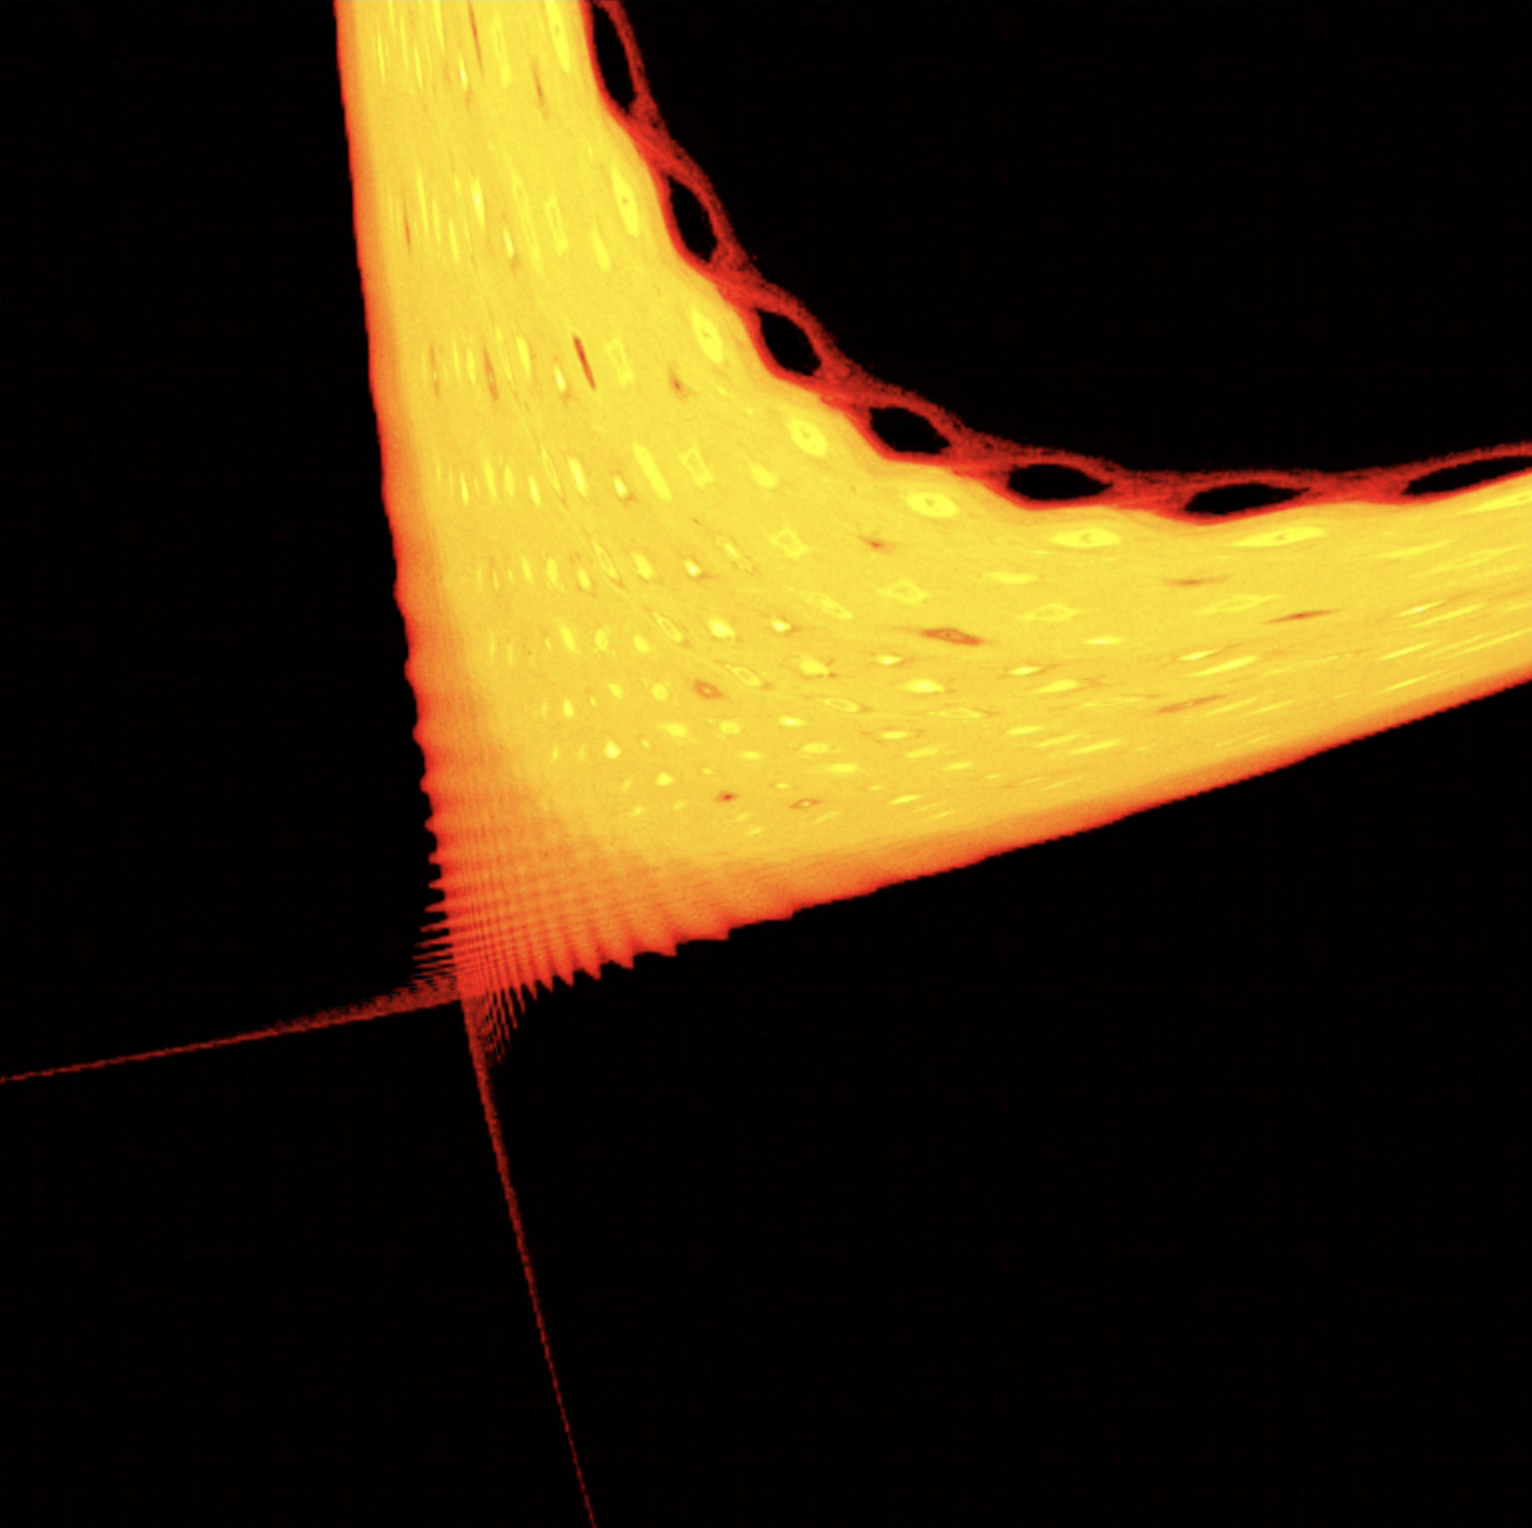
\includegraphics[width=0.49\linewidth]{poincare1}
  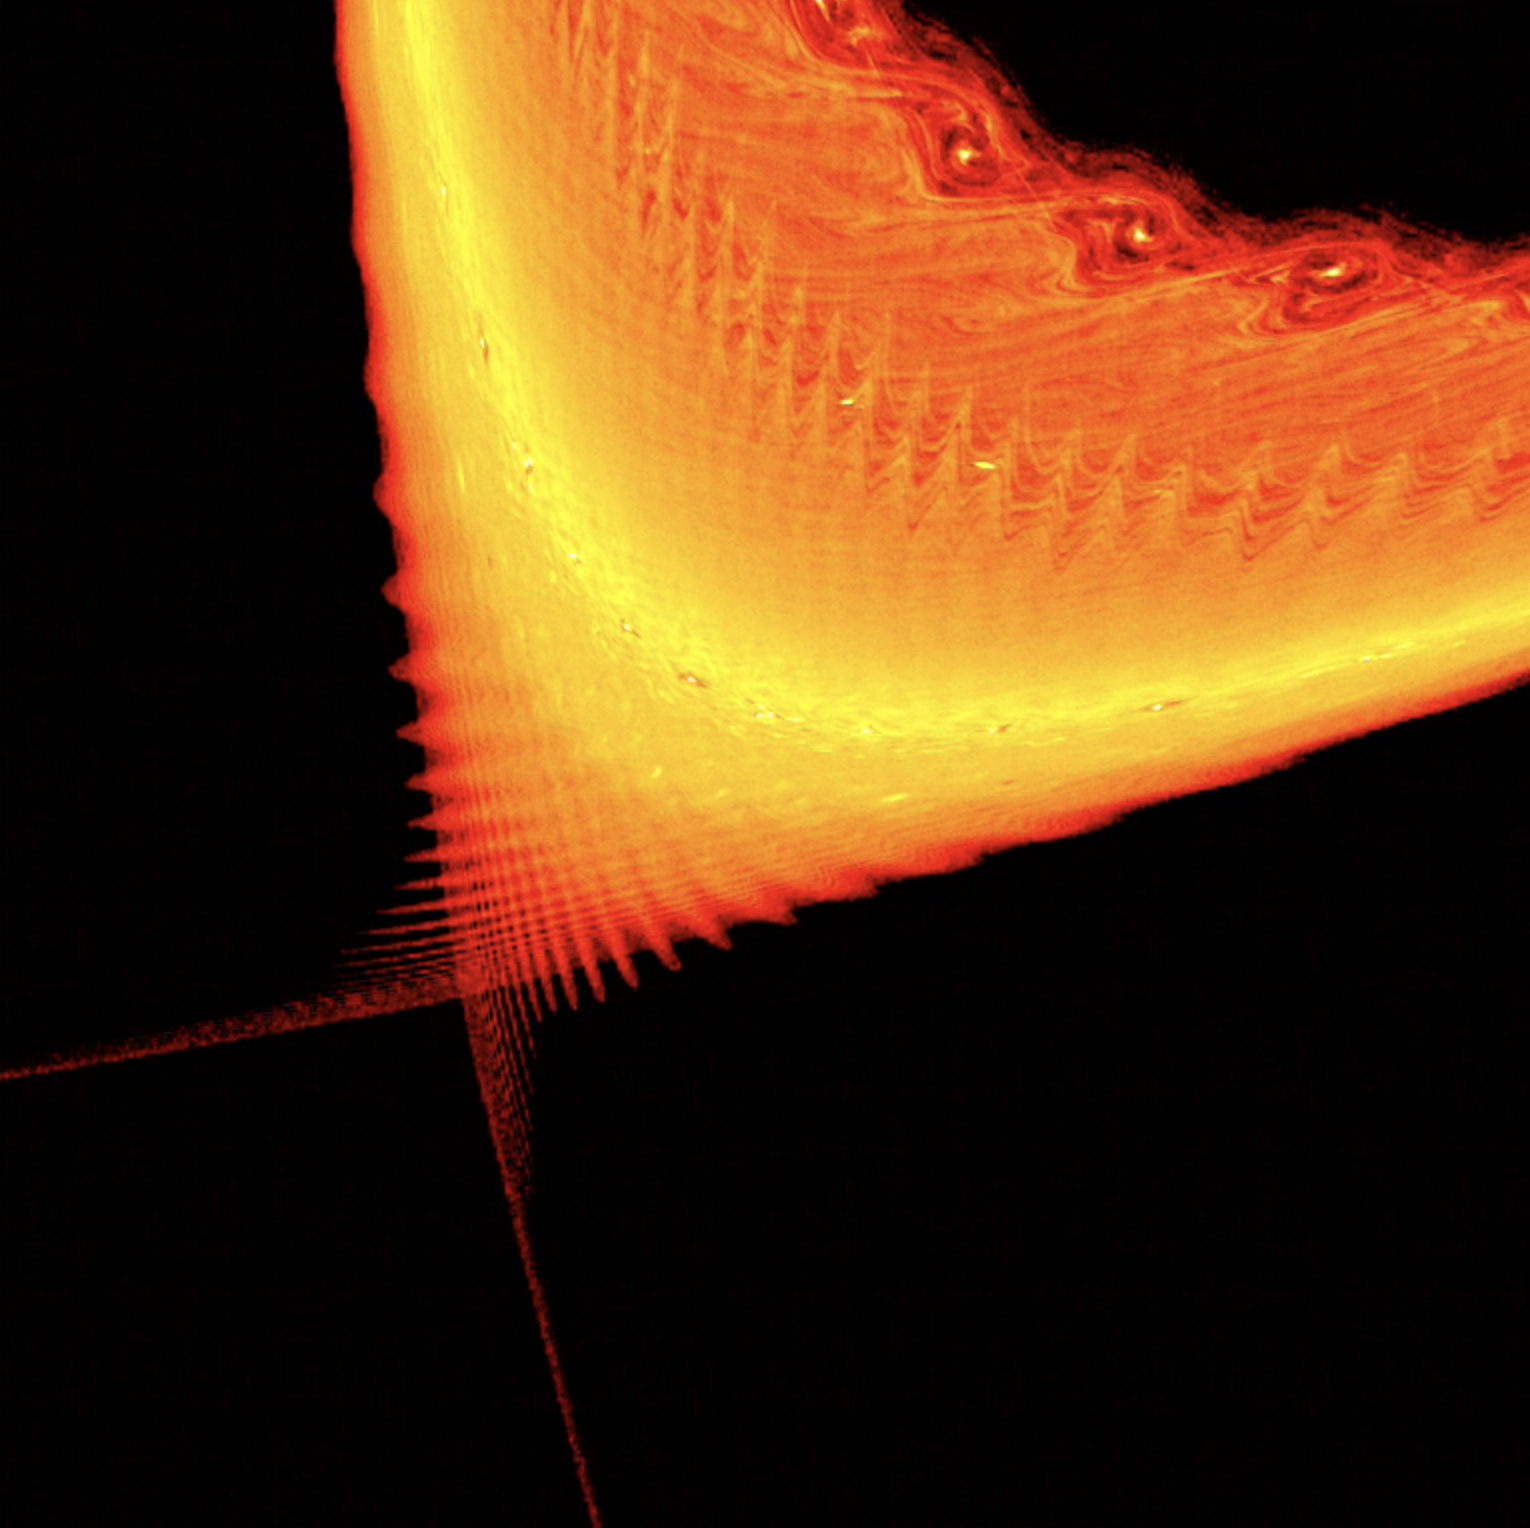
\includegraphics[width=0.49\linewidth]{poincare2}
  \caption{\poincare maps from two different time steps from a simulation run at the Oak Ridge Leadership Computing Facility generated by \vtkm.  The particles were placed near the edge of the tokamak where the plasma becomes very turbulent. The \poincare map shows magnetic features in the plasma as the simulation progresses. Of particular interest are the long fingers that appear in the lower portion of the image. The evolving shape of these fingers over time provides valuable insight into the behavior of the magnetic field where the turbulence is extremely high. }
  \label{fig:poincare}
\end{figure*}

The behavior and evolution of the magnetic field in a tokamak is complex, and its control is critical for performance.
For these reasons, analysis tools used for understanding the dynamic nature of the magnetic field are critical.
The complexity of the 3D magnetic field lines makes analysis and visualization difficult.
Because the field lines are periodic, this complexity can be reduced by using a \poincare magnetic field-line puncture map~\citep{Sanderson2010}. 
The \poincare map is the intersection of a field line with a lower-dimensional subspace (called the \poincare section).
In our case, the \poincare section is a 2D plane that is perpendicular to the axis of the tokamak.
Given a set of magnetic field lines, the \poincare map (i.e., the intersection of the magnetic field lines with the plane) provides a concise 
representation of the magnetic field and is easier to understand and analyze.
Figure~\ref{fig:poincare} shows some examples of \poincare plots generated by \vtkm.

In practice, the \poincare map is generated by creating many field lines and plotting each intersection, or puncture, with the plane.
After a sufficient number of punctures has been collected, patterns in the map characterize the features in the magnetic field.
The field lines are computed by modeling massless particles that follow magnetic field lines.
These massless particles can follow magnetic field lines by advecting them in the direction of the magnetic field.
The intersections generated from a single particle characterize the features of the magnetic surface at that position.
The particles are advected using a differential equation solver such as the fourth order Runge-Kutta scheme.

Proper characterization of the magnetic field requires a large number of initial positions (typically tens of thousands), each of which typically results in between 1,000 and 3,000 intersections, with each intersection following a field line all the way through the tokamak's torus.
Because of these numerous features, the computation of a \poincare map can be very expensive.
The WDMApp team has a \poincare map code that runs on CPUs and takes several hours for the largest analysis run. 
%Because of this cost, the generation \poincare maps required careful planning.
The high cost of the analysis is due to two main factors: (1) the many particles and intersections required and (2) the complexity of the magnetic field calculation.  In many applications of particle advection, the vector field is calculated at the nodes of each cell in the mesh. Linear interpolation within the cell is used to evaluate the magnetic field for the particle being advected. Because of the large number of advection steps required for each particle in the \poincare map, small errors can rapidly accumulate. These errors are compounded because the evaluation of the magnetic field requires a complex set of calculations, and these calculations require high-order interpolation of several quantities.

Using \vtkm can significantly accelerate the computation of \poincare maps by leveraging the parallelism of GPUs. Because the trajectory of each particle is completely independent, the task can be parallelized over each particle. Using this approach, a \poincare map can be computed in under $3$ minutes. The wall-clock time for a typical WDMApp simulation step is between $1.5$ and $2$ minutes, which means that \poincare maps can be computed in situ in nearly real time.
When WDMApp is run, the EFFIS workflow control system~\citep{Suchyta2022:effis} allocates an additional 1--2 nodes for the \poincare map analysis. As a simulation step completes, EFFIS launches a \poincare analysis task on GPUs in the node in a round-robin fashion. This allows asynchronous analysis to be performed on the additional nodes while the simulation is running.
Because EFFIS was already being used as a code-integrating technology, it was straightforward to integrate \vtkm directly into this system.
Figure~\ref{fig:poincare} shows \poincare maps from two different time steps of a simulation run at the OLCF.
Real-time generation of \poincare maps provides the WDMApp team with unprecedented capability for analysis of magnetic fields in fusion simulations.


\subsection{Impact beyond ECP}

%\assign{Jay}

%\jay{discuss the applications/use cases outside of ECP}
In addition to the applications mentioned above, \vtkm still serves as the key infrastructure for accelerating data analysis and visualization in various scientific applications through in-situ visualization. This subsection lists several examples and illustrates how \vtkm is integrated into in-situ scientific workflows outside of the ECP.


\begin{figure}[htb]
  \centering
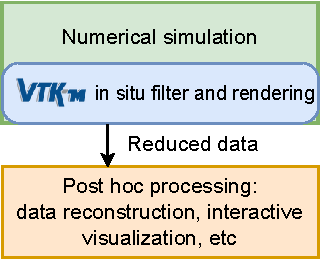
\includegraphics[width=0.60\linewidth]{vtkm_insitu_posthoc}
\caption{The in-situ reduction + post-hoc paradigm based on \vtkm.}
\label{fig:vtkm_insitu_posthoc}
\end{figure}

Before being selected as a project in the ECP, \vtkm was a core component in the Visualization for the Extreme-Scale Scientific Computation Ecosystem (XVis)~\citep{Moreland2019} project. 
XVis focused on multiple ways to integrate in-situ visualization with the simulation, extract key information, and decrease the data size for post-hoc processing.
The \textit{in-situ reduction + post hoc} paradigm (Figure~\ref{fig:vtkm_insitu_posthoc}) is adopted in multiple scientific domains within and outside of the ECP, such as probability distribution function extraction of fields in combustion simulation~\citep{Ye2016} and binning mechanisms to reduce the data size of fusion simulation~\citep{Kress2018}. We use two recent efforts as examples to illustrate how \vtkm facilitates scientific workflows beyond the ECP.


Nyx is a cosmological simulation code that aims to solve compressible hydrodynamics with $N$-body treatment of dark matter. Each simulation run may contain hundreds of time steps with multiple sets of simulation input parameters. The raw data size is usually hundreds of terabytes to several petabytes---a size that presents challenges when post-processing the data. 
\vtkm is used for in-situ analysis to extract the statistical properties of the down-sampled data to significantly reduce the size of raw data. The associated statistics model can be used to construct the data based on prior knowledge in post-processing with low data reconstruction error~\citep{Wang2019}.

Eddy detection and tracking play key roles in analyzing the data generated by ocean simulations. Understanding the characteristics of eddies can help scientists explain the regional air-sea interactions.
The \vtkm streamline filter can be used as an in-situ analysis to generate streamline data used for interactive post-hoc analysis~\citep{Han2022}. With the help of \vtkm, the associated eddy analysis workflow can improve the interaction speed, reduce data storage, and meet the
needs of real-time visual analysis interaction.  

% TODO, add a summary figure, altough not use ECP solution, vtk-m play key role in developing insitu solution
